\documentclass{beamer}
\usetheme{Madrid}

\usepackage{cmap}
\usepackage[T2A]{fontenc}
\usepackage[russian,english]{babel}
\usepackage[utf8]{inputenc}
\usepackage{amsmath, amssymb}
\usepackage{minted}
\usepackage{hologo}

\usepackage{algorithm2e}
\usepackage{algorithmic}
\usepackage{float}

\usepackage{cancel}
\usepackage{ulem}

% \newtcbox{\mybox}{blank, on line, opacitytext=0.5}

\title[Ускорение обучения языковых моделей]{Методы предобработки текстовых данных для ускорения обучения языковых моделей с помощью обучения по плану}

\author[Сурков М.К.]{Сурков Максим Константинович\\
 	{\footnotesize Научный руководитель: Ямщиков Иван Павлович}
}
\institute[НИУ ВШЭ СПБ]{Санкт-Петербургская школа физико-математических и компьютерных наук \\ НИУ ВШЭ СПБ}
\date{20 апреля 2021 г.}

\begin{document}

\frame{\titlepage}

\begin{frame}
	\frametitle{Мотивация. Применения}
	\begin{columns}
		\column{0.5\textwidth}
		\begin{itemize}
			\item социальные сети
			\item голосовые помощники
			\item переводчики
			\item чат-боты
		\end{itemize}
		\column{0.5\textwidth}
		
\includegraphics[scale=0.2]{nlp_real_life.png}
	\end{columns}
	\noindent\makebox[\linewidth]{\rule{\paperwidth}{0.4pt}}
	\begin{columns}
		\column{0.5\textwidth}
		\begin{itemize}
			\item классификация
			\item машинный перевод
			\item вопросно-ответные системы
		\end{itemize}
		\column{0.5\textwidth}
		\begin{itemize}
			\item небольшие языковые модели
			\item GPT-3
			\begin{itemize}
				\item очень большая модель
			\end{itemize}
			\item {\bf BERT}
			\begin{itemize}
				\item высокое качество
			\end{itemize}
		\end{itemize}
	\end{columns}
\end{frame}

\begin{frame}
	\frametitle{Мотивация. Обучение языковой модели}
	\begin{itemize}
		\item текст $\rightarrow$ токены $\rightarrow$ BERT $\rightarrow$ предсказание
	\end{itemize}
	
\includegraphics[scale=0.4]{pre_training_fine_tuning.png}
	\begin{columns}
		\column{0.5\textwidth}
			\begin{itemize}
				\item требуемое время: от 1-2 дней до {\bf 1-2 недель}
				\item мировой рекорд: 47 минут с использованием {\bf 1472} GPU

				\begin{table}
					\begin{tabular}{l|c}
						Корпус данных & Размер \\
						\hline\hline
						Wikipedia & 3-600M \\
						BookCorpus & 74M\\
					\end{tabular}
				\end{table}
			\end{itemize}
		\column{0.5\textwidth}
			\begin{itemize}
				\item требуемое время: 1-2 дня

				\begin{table}
					\begin{tabular}{l|c}
						Корпус данных & Размер \\
						\hline\hline
						HND & 600k-2M \\
						s140 & 1.6M \\
						IWSLT & 200-230k \\
						QQP & 364k \\
						MNLI & 393k \\
					\end{tabular}
				\end{table}
			\end{itemize}
	\end{columns}
	\noindent\makebox[\linewidth]{\rule{\paperwidth}{0.4pt}}
	\begin{itemize}
		\item {\bf долго} обучать
		\item нужно обрабатывать {\bf большие} объемы данных
	\end{itemize}
\end{frame}

\begin{frame}
	\frametitle{Обучение по плану. Определение}
	\begin{columns}
		\column{0.5\textwidth}
		\begin{enumerate}
			\item сортируем данные по сложности (длина)
			\item в течение $T$ шагов (рассмотрим $t$-й шаг)
			\begin{itemize}
				\item вычисляем $c(t) \in [0, 1]$
				\item формируем пакет данных маленького размера из множества $c(t)$ {\bf легких} примеров
				\item шаг обучения
			\end{itemize}
		\end{enumerate}
		\column{0.5\textwidth}
		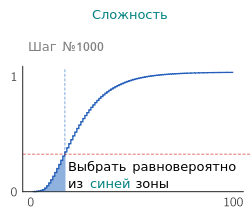
\includegraphics[scale=0.8]{acl19_algo.png}
	\end{columns}
	\let\thefootnote\relax\footnotetext{Platanios et al., Competence-based Curriculum Learning for
		Neural Machine Translation, 2019}
\end{frame}

\begin{frame}
	\frametitle{Метод сравнения алгоритмов обучения}
	\begin{columns}
		\column{0.5\textwidth}
		\begin{enumerate}
			\item фиксируем: корпус данных, модель, семплер
			\item обучаем модель
			\item фиксируем достаточно большой порог (точность, функция потерь)
			\item сравниваем среднее число шагов, необходимое для достижения данного порога
		\end{enumerate}
		\column{0.5\textwidth}
		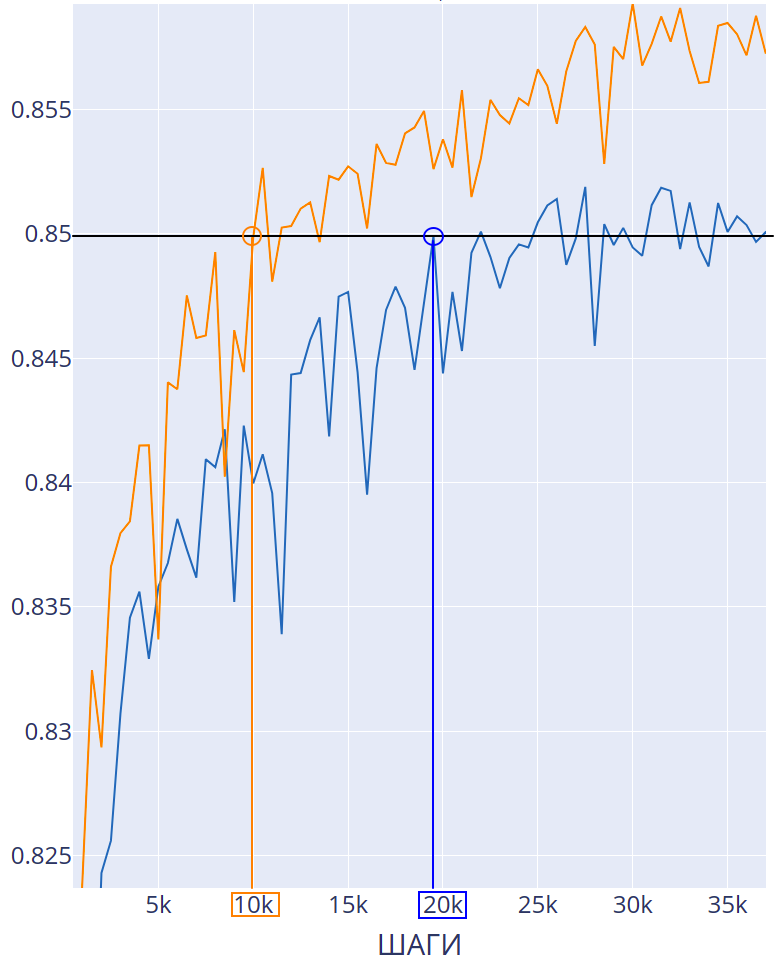
\includegraphics[scale=0.25]{compare}
	\end{columns}
\end{frame}

\begin{frame}
	\frametitle{Поле исследований}
	\begin{table}
		\begin{tabular}{l|cccc}
			метрика & классификация & перевод & предобучение & NLU \\
			\hline
			длина & & $\checkmark$ & & \\
			{\it языковая}\footnote[1]{Sluis et al. (2010) показали слабую корреляцию с реальной сложностью текста} & & & & \\
			энтропия & & & & \\
			модельная & & & & $\checkmark$ \\
			частота слов & & $\checkmark$ & & \\
			правдоподобие & & $\checkmark$ & & \\
			\hline
		\end{tabular}
	\end{table}
	\begin{itemize}
		\item не изучено влияние обучения по плану на задачах {\bf классификации и предобучения}
		\item покрыто {\bf узкое} множество метрик (длина - лучшая метрика на данный момент)
		\item большинство работ улучшают {\bf качество} модели, но {\bf не скорость} обучения
		\item не рассмотрен случай с {\bf шумными} тренировочными данными
	\end{itemize}
\end{frame}

\begin{frame}
	\frametitle{Цель и задачи}
	{\bf Цель:} ускорить обучение языковой модели BERT с помощью обучения по плану за счет применения улучшенной метрики сложности текстовых данных на задачах классификации и предобучения
	
	{\bf Задачи:}
	\begin{enumerate}
		\item Предложить метрики оценки сложности текста
		\item Реализовать производительные алгоритмы вычисления предложенных метрик на больших корпусах данных
		\item Сравнить найденные метрики
		\item Исследовать влияние найденных метрик на скорость обучения языковой модели BERT на чистых и шумных тренировочных данных
	\end{enumerate}
\end{frame}

\begin{frame}
	\frametitle{Поиск метрик}
	\begin{enumerate}
		\item  база
		\begin{itemize}
			\item {\bf длина}, вероятность правдоподобия (Platanios et al., 2019)
			\item самое редкое слово в предложении (Xuan Zhang et al., 2018)
		\end{itemize}
		\item информационный поиск
		\begin{itemize}
			\item {\bf tf-idf}
		\end{itemize}
		\item {\bf теория информации} (Nihat Ay et al., 2006)
		\begin{itemize}
			\item EE, TSE
				\begin{columns}
					\column{0.5\textwidth}
					\[
					T=(t_1, t_2, \ldots, t_{i-1},t_i,\ldots, t_n)
					\]
					\[
					\downarrow
					\]
					\[
					\xi=(\xi^1_{t_1},\xi^2_{t_2},\ldots,\xi^{i-1}_{t_{i-1}},\xi^i_{t_i},\ldots,\xi^n_{t_n})
					\]
					\[
					t_i\rightarrow \xi^i_{t_i} =: \mu_i - \text{бинарная случайная величина}
					\]
					\column{0.5\textwidth}
					\begin{table}
					\begin{tabular}{|c|c|}
					\hline
					Асимптотика & Время \\
					\hline
					$\mathcal{O^*}(2^n), \mathcal{O}(n^2)$ & > 1 мес. \\
					\hline
					$\mathcal{O}(n)$ & < 4ч. \\
					\hline
					\end{tabular}
					\end{table}
				\end{columns}
		\end{itemize}
		\item модельная (MLM-loss)
		\begin{itemize}
			\item
			учим BERT на задаче MLM (Пример: "Привет, как [МАСКА]?"), оптимизируя кросс-энтропию
			\item сложность = значение кросс-энтропии на данном тексте
			\item треубет GPU
		\end{itemize}
		\item среднее число токенов в слове (TPW)
	\end{enumerate}
\end{frame}

\begin{frame}
	\frametitle{Вычисление метрик}
	\begin{itemize}
		\item статистики
			\begin{enumerate}
				\item длина $\rightarrow$ число текстов с такой длиной
				\item $(i, x_i) \rightarrow$ число текстов, где $t_i = x_i$ 
				\item $(x_i)\rightarrow$ число текстов, где $x_i$ является последним токеном
				\item $(i, x_{i-1}, x_i) \rightarrow$ число текстов, где на $(i-1)$-й позиции стоит $x_{i-1}$, а на $i$-й позиции стоит $x_i$
				\item $x_i \rightarrow$ число текстов, в которых есть $x_i$
			\end{enumerate}
		\item сбор статистик в параллельном режиме (разделение по данным)
			\begin{table}
				\begin{tabular}{|c|c|}
					\hline
					Режим & Время \\
					\hline
					1 CPU & $\approx$ 2 недели \\
					5 CPU & $\approx$ 1-2 дня \\
					20 CPU & < 6 ч. \\
					\hline
				\end{tabular}
			\end{table}
	\end{itemize}
	\noindent\makebox[\linewidth]{\rule{\paperwidth}{0.4pt}}
	Итого:
	\begin{itemize}
		\item предложены подходы, покрывающие широкое множество метрик
		\item предложены алгоритмы, вычисляющие метрики за пренебрежимо маленькое время ($<8\%$ от времени обучения)
	\end{itemize}
\end{frame}

\begin{frame}
	\frametitle{Сравнение метрик. Предобучение}
	\begin{columns}
		\column{0.5\textwidth}
			\begin{itemize}
				\item Данные: 
				
					Wikipedia, BookCorpus
				\item Обучение по плану проигрывает базовому решению от 2 до 5 раз
				\item Метрики имеют порядок вне зависимости от семплера
				\begin{enumerate}
					\item {\bf максимальный ранг слова}
					\item TF-IDF
					\item EE
					\item TSE
					\item правдоподобие
					\item {\bf длина}
				\end{enumerate}
				\item Длина проигрывает остальным метрикам от 2 до 12 раз
			\end{itemize}
		\column{0.5\textwidth}
			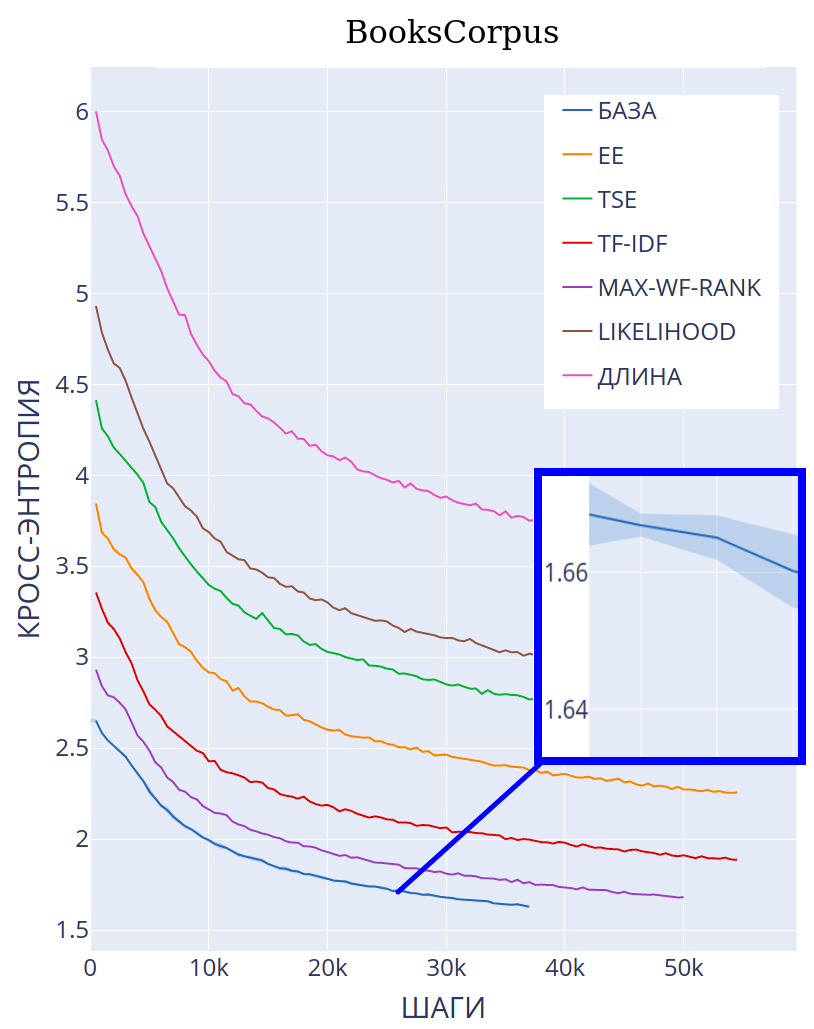
\includegraphics[scale=0.28]{BookCorpus_results}
	\end{columns}
\end{frame}

\begin{frame}
	\frametitle{Сравнение метрик. Предобучение}
	$\max\Delta \le 3k$
	\begin{table}
		\begin{tabular}{l|ccccc|c}
			Корпус данных & \multicolumn{5}{c}{BookCorpus (2.00)}\\
			\hline
			семплер & CB & DB & Hyp & SS & SM & min loss\\
			\hline
			max wf rk & $\infty$ & 17.5k & {\bf 16.5k} & {\bf 16.5k} & 27k & {\bf 1.58} \\
			TF-IDF & $\infty$ & 34k & 35k & 37.5k & $\infty$ & 1.84 \\
			\hline
			база & \multicolumn{5}{c}{9.5k} & 1.58 \\
			\hline
			\hline
			& \multicolumn{5}{c}{BookCorpus (3.50)}\\
			\hline
			EE & $\infty$ & 4k & 3.5k & 4.5k & 9.5k & 2.25 \\
			TSE & $\infty$ & 9k & 9k & 8.5k & 18k & 2.60 \\
			правдоподобие & $\infty$ & 13.5k & 13.5k & 15.5k & 50k & 2.83 \\
			длина & $\infty$ & 50.5k & $\infty$ & - & - & 3.45 \\
			\hline
		\end{tabular}
	\end{table}
	\begin{itemize}
		\item {\bf\color{orange}$(\pm)$} лучшая метрика -- максимальный ранг слова ({\bf\color{red}$(-)$}замедляет в $2$ раза {\bf\color{green}$(+)$} {\bf без потери качества})
		\item {\bf\color{red}$(-)$} обучение по плану замедляет обучение от 2 до 5 раз и ухудшает качество модели
	\end{itemize}
\end{frame}

\begin{frame}
	\frametitle{Сравнение метрик. Классификация}
	$\max\Delta \le 3k$
	\begin{table}
		\begin{tabular}{l|ccccc|c}
			Корпус данных & \multicolumn{5}{c}{sentiment140 (85.5\%)}\\
			\hline
			семплер & CB & DB & Hyp & SS & SM & Точность\\
			\hline
			длина & 112.5k & 20k & 19k & - & - & {\bf 86.2\%} \\
			TF-IDF & 115.5k & 21.5k & 19.5k & {\bf 16.5k} & 22k & 86.7\% \\
			TSE & 95.5k & {\bf 16.5k} & 20.5k & 21.5k & 18k & 86.8\% \\
			EE & 59k & 19.3k & 23k & 20k & 19k & 86.7\% \\
			max wf rk & 70k & 18.5k & 19.5k & {\bf 17k} & 19k & 86.7\% \\
			правдоподобие & 112k & {\bf 17.5k} & 21.5k & {\bf 17.5k} & 21.5k & 86.7\% \\
			MLM-loss & 59.5k & 21k & 23.5k & ? & ? & {\bf 86.1\%} \\
			\hline
			база & \multicolumn{5}{c}{17.5k} & 87\%
		\end{tabular}
	\end{table}
	\begin{itemize}
		\item {\bf\color{green}$(+)$} лучшая конфигурация (TF-IDF+SS) ускоряет обучение до 3\% в среднем
		\item {\bf\color{red}$(-)$} длина и MLM-loss уменьшают точность модели на 0.6\%
		\item {\bf\color{red}$(-)$} нет значительного ускорения обучения
	\end{itemize}
\end{frame}

\begin{frame}
	\frametitle{Влияние метрик на скорость обучения. Шум}
	\begin{itemize}
		\item $p \sim U[0, 0.4]$ -- уровень шума (доля слов с шумом)
			\begin{itemize}
				\item {\bf искусственная} метрика
			\end{itemize}
		\item виды шума:
			\begin{enumerate}
				\item вставки
				\item удаления
				\item {\bf клавиатурный}
			\end{enumerate}
	\end{itemize}
%	\noindent\makebox[\linewidth]{\rule{\paperwidth}{0.4pt}}
	\begin{columns}
		\column{0.5\textwidth}
		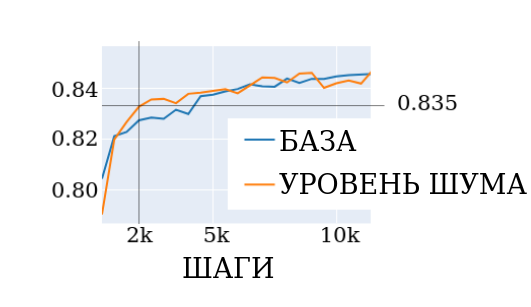
\includegraphics[scale=0.48]{keyboard_noise_level_short_prefix}
		метрика "уровень шума" ускоряет обучение на старте до 2.5 раз
		\column{0.5\textwidth}
		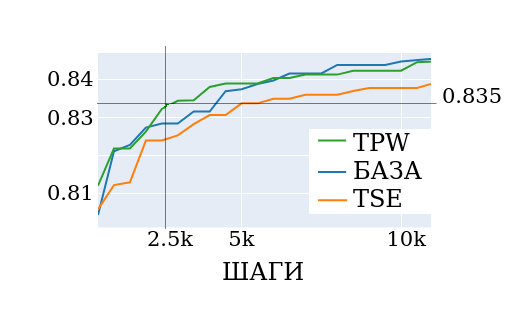
\includegraphics[scale=0.5]{keyboard_noise_TPW_win}
		{\bf\color{green}$(+)$} метрика TPW ускоряет обучение до 2 раз на первых 10\% всего обучения
	\end{columns}
\end{frame}

\begin{frame}
	\frametitle{Результаты}
	\begin{enumerate}
		\item Предложен широкий спектр метрик оценки сложности текста
		\begin{itemize}
			\item метрики TSE и EE адаптированы под задачу обработки языка
		\end{itemize}
		\item Реализованы алгоритмы подсчета метрик на больших объемах данных ($\le 8\%$ от времени обучения)
		\item Предобучение
			\begin{itemize}
				\item {\bf\color{green}$(+)$} есть строгий порядок метрик
				\item {\bf\color{red}$(-)$} длина -- худшая метрика на предобучении (замедляет обучения до 12 раз, уменьшает качество модели)
				\item максимальный ранг слова -- лучшая метрика на предобучении ({\bf\color{red}$(-)$}замедляет в $2$ раза {\bf\color{green}$(+)$} {\bf без потери качества})
			\end{itemize}
		\item Классификация
			\begin{itemize}
				\item {\bf\color{green}$(+)$} лучшая конфигурация (TF-IDF+SS) ускоряет обучение до 3\% в среднем на классификации
				\item {\bf\color{red}$(-)$} длина и MLM-loss уменьшают точность модели на 0.6\%
				\item 
				{\bf\color{green}$(+)$} метрика TPW ускоряет обучение до {\bf 2 раз} на первых 10\% всего обучения на шумном корпусе данных
			\end{itemize}
	\end{enumerate}
\end{frame}

\appendix

\begin{frame}[label=supplemental,noframenumbering]
	\frametitle{Дополнительно: ссылки}
	\begin{itemize}
		\item Ay, N., Olbrich, E., Bertschinger, N., \& Jost, J. (2006, August). A\\\hspace{1cm}unifying framework for
		complexity measures of finite systems. In\\\hspace{1cm}Proceedings of ECCS (Vol. 6).
		\item Bengio, Y., Louradour, J., Collobert, R., \& Weston, J. (2009, June).\\\hspace{1cm}Curriculum learning. In
		Proceedings of the 26th annual \\\hspace{1cm}international conference on machine learning (pp.
		41-48).
		\item Brown, T. B., Mann, B., Ryder, N., Subbiah, M., Kaplan, J., \\\hspace{1cm}Dhariwal, P., ... \& Amodei, D.
		(2020). Language models are\\\hspace{1cm}few-shot learners. arXiv preprint arXiv:2005.14165.
		\item Devlin, J., Chang, M. W., Lee, K., \& Toutanova, K. (2018). Bert: \\\hspace{1cm}Pre-training of deep
		bidirectional transformers for language\\\hspace{1cm} understanding. arXiv preprint
		arXiv:1810.04805.
	\end{itemize}
\end{frame}

\begin{frame}[label=supplemental,noframenumbering]
	\frametitle{Дополнительно: ссылки}
	\begin{itemize}
		\item Hacohen, G., \& Weinshall, D. (2019, May). On the power of \\\hspace{1cm}curriculum learning in training
		deep networks. In International\\\hspace{1cm}Conference on Machine Learning (pp. 2535-2544).
		PMLR.
		\item Kocmi, T., \& Bojar, O. (2017). Curriculum learning and minibatch \\\hspace{1cm}bucketing in neural
		machine translation. arXiv preprint \\\hspace{1cm}arXiv:1707.09533.
		\item Kurdi, M. Z. (2020). Text Complexity Classification Based on \\\hspace{1cm}Linguistic Information:
		Application to Intelligent Tutoring of \\\hspace{1cm}ESL. arXiv preprint arXiv:2001.01863.
		\item Mermer, M. N., \& Amasyali, M. F. (2017). Scalable Curriculum \\\hspace{1cm}Learning for Artificial
		Neural Networks. IPSI BGD \\\hspace{1cm}TRANSACTIONS ON INTERNET RESEARCH, 13(2).
	\end{itemize}
\end{frame}

\begin{frame}[label=supplemental,noframenumbering]
	\frametitle{Дополнительно: ссылки}
	\begin{itemize}
		\item Narasimhan, S., Narasimhan, V. A. P. B. S., Karch, G., Rao, R., \\\hspace{1cm}Huang, J., Zhang, Y.,
		Ginsburg, B., Chitale, P., Sreenivas, S., \\\hspace{1cm}Mandava, S., Ginsburg, B., Forster, C., Mani,
		R., \& Kersten, K. \\\hspace{1cm}(2020, October 13). NVIDIA Clocks World’s Fastest BERT \\\hspace{1cm}Training
		Time and Largest Transformer Based Model, Paving \\\hspace{1cm}Path For Advanced
		Conversational AI. NVIDIA Developer Blog.
		\\\hspace{1cm}https://developer.nvidia.com/blog/training-bert-with-gpus/
		\item Platanios, E. A., Stretcu, O., Neubig, G., Poczos, B., \& Mitchell, T. \\\hspace{1cm}M. (2019).
		Competence-based curriculum learning for neural \\\hspace{1cm}machine translation. arXiv preprint
		arXiv:1903.09848.
		\item Sajjad, H., Dalvi, F., Durrani, N., \& Nakov, P. (2020). Poor Man's \\\hspace{1cm}BERT: Smaller and Faster
		Transformer Models. \\\hspace{1cm}arXiv preprint arXiv:2004.03844.
	\end{itemize}
\end{frame}


\begin{frame}[label=supplemental,noframenumbering]
	\frametitle{Дополнительно: ссылки}
	\begin{itemize}
		\item Shen, S., Dong, Z., Ye, J., Ma, L., Yao, Z., Gholami, A., Mahoney, M. \\\hspace{1cm}W., \& Keutzer, K.
		(2020). Q-BERT: Hessian Based Ultra Low \\\hspace{1cm}Precision Quantization of BERT.
		Proceedings of the AAAI \\\hspace{1cm}Conference on Artificial Intelligence, 34(05), 8815–8821.
		\\\hspace{1cm}https://doi.org/10.1609/aaai.v34i05.6409
		\item van der Sluis, F., \& van den Broek, E. L. (2010, August). Using \\\hspace{1cm}complexity measures in
		information retrieval. In Proceedings of \\\hspace{1cm}the third symposium on information
		interaction in context (pp. \\\hspace{1cm}383-388).
		\item Vaswani, A., Shazeer, N., Parmar, N., Uszkoreit, J., Jones, L., Gomez, \\\hspace{1cm}A. N., ... \&
		Polosukhin, I. (2017). Attention is all you need. \\\hspace{1cm}arXiv preprint arXiv:1706.03762.
	\end{itemize}
\end{frame}

\begin{frame}[label=supplemental,noframenumbering]
	\frametitle{Дополнительно: ссылки}
	\begin{itemize}
		\item Xu, B., Zhang, L., Mao, Z., Wang, Q., Xie, H., \& Zhang, Y. (2020). \\\hspace{1cm}Curriculum Learning for
		Natural Language Understanding. \\\hspace{1cm}Proceedings of the 58th Annual Meeting of the
		Association for \\\hspace{1cm}Computational Linguistics, 6095–6104.
		\\\hspace{1cm}https://doi.org/10.18653/v1/2020.acl-main.542
		\item Zhang, X., Kumar, G., Khayrallah, H., Murray, K., Gwinnup, J., \\\hspace{1cm}Martindale, M. J., ... \&
		Carpuat, M. (2018). An empirical \\\hspace{1cm}exploration of curriculum learning for neural
		machine \\\hspace{1cm}translation. arXiv preprint arXiv:1811.00739.
	\end{itemize}
\end{frame}

\begin{frame}[label=supplemental,noframenumbering]
	\frametitle{Дополнительно: Поиск метрик}
	\let\thefootnote\relax\footnotetext{Nihat Ay et al., A {\bf Unifying }Framework for Complexity Measures of Finite Systems, 2006}
	
	\begin{table}
		\begin{tabular}{c|c}
			\hline
			метрика & формула \\
			\hline
			Мультиинформация & $\sum\limits_{v\in V}H_p(X_v) - H_p(X_V)$ \\
			\hline
			{\bf Избыточная энтропия (EE)} & $\left[\sum\limits_{v\in V}H(X_{V\backslash\{v\}})\right] - (n - 1)H(X_V)$ \\
			\hline
			{\bf TSE} & $\sum\limits_{k=1}^{n-1}\frac{k}{n}C^{(k)}(X_V)$, где \\\\
			& $C^{(k)}(X_V) =$ \\\\
			& $\frac{n}{k\binom{n}{k}}\sum\limits_{A\subseteq V,|A|=k}H(X_A) - H(X_V)$ \\
			\hline
			Переходная информация & :( \\
			\hline
		\end{tabular}
	\end{table}
	
	\[
	V=\{1,\ldots,n\},
	X_V = (X_1,\ldots,X_n)
	\]
\end{frame}

\begin{frame}[label=supplemental,noframenumbering]
	\frametitle{Дополнительно: Адаптация EE и TSE под задачи обработки языка}
	
	\begin{enumerate}
		\item Образование совместной случайной величины
		\[
		T=(t_1, t_2, \ldots, t_{i-1},t_i,\ldots, t_n)
		\]
		\[
		t_i\rightarrow \xi^i_{t_i} =: \mu_i - \text{бинарная случайная величина}
		\]
		\[
		\downarrow
		\]
		\[
		\xi=(\xi^1_{t_1},\xi^2_{t_2},\ldots,\xi^{i-1}_{t_{i-1}},\xi^i_{t_i},\ldots,\xi^n_{t_n})
		\]
		\item Вычисление энтропии
		\[
		H(\mu) = \sum\limits_{i=1}^{n}H(\mu_i|\mu_1,\mu_2,\ldots,\mu_{i-1}) = \sum\limits_{i=1}^{n}H(\mu_i|\mu_{i-L},\ldots,\mu_{i-1})
		\]
		\item $L=1$
		\[
		H(\mu) = H(\mu_1) + H(\mu_2|\mu_1) + \ldots + H(\mu_i|\mu_{i-1}) + \ldots + H(\mu_n|\mu_{n-1})
		\]
	\end{enumerate}
\end{frame}

\begin{frame}[label=supplemental,noframenumbering]
	\frametitle{Дополнительно: Вычисление EE}
	\[
	EE(X) = \left[\sum\limits_{v\in V}H(X_{V\backslash\{v\}})\right] - (n - 1)H(X_V) = 
	\]
	\[
	\left[\sum\limits_{i=1}^{n}H(\mu_1,\ldots,\mu_{i-1},\mu_{i+1},\ldots,\mu_n)\right] - (n - 1)H(\mu)
	\]
	\begin{itemize}
		\item $\mathcal{O}(n^2)$
		\item $\mathcal{O}(n)$
		\[
		\sum\limits_{i=1}^{n}H(\mu_1,\ldots,\mu_{i-1},\mu_{i+1},\ldots,\mu_n) =\]
		\[ = \sum\limits_{i=1}^{n}H(\mu) - H(\mu_i|\mu_{i-1}) - H(\mu_{i+1}|\mu_i) + H(\mu_{i+1})\]
		\[
		EE(X) = \sum\limits_{i=2}^{n}H(\mu_i) - H(\mu_i|\mu_{i-1})= \sum\limits_{i=2}^{n}I(\mu_{i-1}\colon\mu_i)
		\]
	\end{itemize}
\end{frame}

\begin{frame}[label=supplemental,noframenumbering]
	\frametitle{Дополнительно: Вычисление TSE}
	\[
	\sum\limits_{k=1}^{n-1}\frac{k}{n}C^{(k)}(X_V)
	\]
	\[
	C^{(k)}(X_V) = \frac{n}{k\binom{n}{k}}\sum\limits_{A\subseteq V,|A|=k}H(X_A) - H(X_V) =
	\]
	\[
	= \frac{n}{k}\left[\frac{1}{\binom{n}{k}}\sum\limits_{A\subseteq V,|A|=k}H(X_A)\right] - H(X_V)
	\]
\end{frame}

\begin{frame}[label=supplemental,noframenumbering]
	\frametitle{Дополнительно: Вычисление TSE}
	\[
	\frac{1}{\binom{n}{k}}\sum\limits_{A\subseteq V,|A|=k}H(X_A) =
	\frac{1}{\binom{n}{k}}\sum\limits_{1 \le i_1 < i_2 < \ldots < i_k \le n}H(\mu_{i_1}, \mu_{i_2}, \ldots, \mu_{i_k})
	\]
	\begin{enumerate}
		\item $\mathcal{O^*}(2^n)$
		\item $\mathcal{O}(n^2)$ - динамическое программирование
		\item $\mathcal{O}(n)$
		\[
		\sum\limits_{i=1}^{n}A_iH(\mu_i) + \sum\limits_{i=2}^{n}B_iH(\mu_i|\mu_{i-1})
		\]
		\[
		A_i = 
		\begin{cases}
		\binom{n-2}{k-1}/\binom{n}{k}=\frac{k(n-k)}{n(n-1)},& i > 1 \\
		\binom{n-1}{k-1}/\binom{n}{k}=\frac k n,& i = 1
		\end{cases}
		\]
		\[
		B_i = \frac{\binom{n-2}{k-2}}{\binom{n}{k}} = \frac{k(k-1)}{n(n-1)}
		\]
	\end{enumerate}
\end{frame}

\begin{frame}[label=supplemental,noframenumbering]
	\frametitle{Результаты. Классификация. HND}
	
	Корпус данных: Hyperpartisan News Detection
	
	$\max\Delta \le 3k$
	\begin{table}
		\begin{tabular}{l|ccccc|c}
			Корпус данных & \multicolumn{5}{c}{HND (92.9\%)}\\
			\hline
			семплер & CB & DB & Hyp & SS & SM & Точность\\
			\hline
			длина & 55k & 23k & 22.5k & - & - & 93.7\% \\
			TF-IDF & $\infty$ & 19.5k & 24k & 23.5k & 33k & 93.5\% \\
			TSE & 56.5k & 21k & 23k & 22k & 31k & 93.8\% \\
			EE & 71.5k & 25.5k & 22.5k & 19.5k & 32.5k & 93.8\% \\
			max wf rk & $\infty$ & 22k & 20.5k & 22.5k & 39k & 93.6\% \\
			правдоподобие & $\infty$ & 20k & 24k & 20k & 30k & 93.8\% \\
			\hline
			база & \multicolumn{5}{c}{22k} & 93.8\%
		\end{tabular}
	\end{table}
\end{frame}

\end{document}